\crefalias{section}{appendix}
\crefalias{subsection}{appendix}

\section{Appendix}

\subsection{Duality with Spectral Norm}
\label{app:dual}

We may first prove~\cref{thm:dual_norm}, and we can then directly derive~\cref{eq:optimal_phi}.

\begin{theorem}\label{thm:dual_norm}
    Nuclear norm $\|\!\cdot\!\|_{*}$ is the dual norm of spectral norm $\|\!\cdot\!\|_{2}$,
    which means
    \[
        \|\mG\|_{*}=\max_{\|T\|_2=1}\langle \mG,\mT\rangle.
    \]

    $\operatorname{msign}(\cdot)$ is the dual map based on $\|\!\cdot\!\|_{2}$, which
    means
    \[
        \operatorname{msign}(\mG)=\underset{\|\mT\|_2=1}{\argmax}\langle \mG,\mT\rangle.
    \]
\end{theorem}

\begin{proof}
    Since $\mG \in \sR^{n\times m}$ has Singular Vector Decomposition $\mG = \mU \mSigma
    \mV^{\top}=\sum_{i=1}^{r}\evsigma_{i}\vu_{i}\vv_{i}^{\top}$ where $\vu_{i}\in\sR
    ^{n}$ and $\vv_{i}\in\sR^{m}$ are left and right singular vectors, we
    have
    \begin{equation}
        \langle \mG,\mT \rangle = \operatorname{tr}(\mG^{\top} \mT)=\operatorname{tr}(\sum_{i=1}^{r} \evsigma
        _{i} \vv_{i} \vu_{i}^{\top} \mT)=\sum_{i=1}^{r} \evsigma_{i}
        \vu_{i}^{\top} \mT \vv_{i}.
    \end{equation}
    With $\|\mT\|_{2}=1$ and $\|\vu_{i}\|_{2}=\|\vv_{i}\|_{2}=1$, we have $\vu_{i}^{\top}
    \mT \vv_{i} \leq \|\mT\|_{2} \|\vu_{i}\|_{2}\|\vv_{i}\|_{2} = 1$, hence
    \begin{equation}
        \label{eq:maximum}\langle \mG,\mT \rangle=\sum_{i=1}^{r} \evsigma_{i} \vu_{i}^{\top}
        \mT \vv_{i} \leq \sum_{i=1}^{r} \evsigma_{i} = \|\mG\|_{*}.
    \end{equation}
    Equality is attained when $\vu_{i}^{\top} \mT \vv_{i} = 1$ for all $i=1,\dots,r$, that
    is when
    \begin{equation}
        \mT = \sum_{i=1}^{r} \vu_{i} \vv_{i}^{\top} = \mU_{[:,:r]}\mV_{[:,:r]}^{\top}=\operatorname{msign}
        (\mG).
    \end{equation}
    Note that for this $\mT$ we indeed have $\|\mT\|_{2}=1$ (its nonzero singular
    values are all equal to $1$), so $\mT$ is feasible and achieves the upper
    bound. Therefore, we have
    \begin{equation}
        \underset{\| \mT \|_2=1}{\argmax}\langle \mG, \mT\rangle =\operatorname{msign}(\mG),
    \end{equation}
    and according to~\cref{eq:maximum}, the maximum value equals $\|\mG\|_{*}$.
\end{proof}



\subsection{Proofs: Localization of the Root of \texorpdfstring{$\boldsymbol{h(\lambda)}$}{h(lambda)}}
\label{app:localization}

In this section, we first prove the localization of the root $\lambda^\star$ to $h(\lambda)=0$, which is required in~\cref{sec:tangent_linearization}. We then present experiments showing that the computational overhead of the proposed $\lambda$-solver is negligible compared to the whole training process.

We first prove~\cref{thm:monotonicity}, from which~\cref{thm:localization} follows.

\begin{theorem}\label{thm:monotonicity}
    The function
    \[
        h(\lambda) = \langle \mTheta, \mPhi^{\star}(\lambda) \rangle= \langle \mTheta
        , \operatorname{msign}(\mG + \lambda \mTheta) \rangle
    \]
    is monotonic non-decreasing in $\lambda$.
\end{theorem}

\begin{proof}
    Recall that the matrix sign function can be equivalently defined as the solution of the spectral-norm constrained maximization as in~\cref{thm:dual_norm}:
    \begin{equation}
        \operatorname{msign}(\mG) = \underset{\|T\|_2=1}{\argmax}\langle \mG, \mT \rangle.
    \end{equation}
    Consider two values $\lambda_{2} > \lambda_{1}$. By the definition of $\mPhi^{\star}(\lambda)$ as the maximizer of $\langle \mG + \lambda \mTheta, \cdot \rangle$, we
    obtain
    \begin{align}
        \langle \mG + \lambda_{1} \mTheta,\mPhi^{\star}(\lambda_{1}) \rangle \geq & \langle \mG + \lambda_{1} \mTheta,\mPhi^{\star}(\lambda_{2}) \rangle \tag*{} \\
        \Rightarrow\quad                                                               & \langle \mG ,\mPhi^{\star}(\lambda_{1}) \rangle + \lambda_{1}\langle \mTheta,\mPhi^{\star}(\lambda_{1}) \rangle \geq \langle \mG ,\mPhi^{\star}(\lambda_{2}) \rangle + \lambda_{1}\langle \mTheta,\mPhi^{\star}(\lambda_{2})\rangle,\label{eq:phi1} \\
        \langle \mG + \lambda_{2} \mTheta,\mPhi^{\star}(\lambda_{2}) \rangle \geq & \langle \mG + \lambda_{2} \mTheta,\mPhi^{\star}(\lambda_{1}) \rangle \tag*{} \\
        \Rightarrow\quad                                                               & \langle \mG ,\mPhi^{\star}(\lambda_{2}) \rangle + \lambda_{2}\langle \mTheta,\mPhi^{\star}(\lambda_{2})\rangle\geq \langle \mG ,\mPhi^{\star}(\lambda_{1}) \rangle+\lambda_{2}\langle \mTheta,\mPhi^{\star}(\lambda_{1})\rangle.\label{eq:phi2}
    \end{align}
    Summing~\cref{eq:phi1} and~\cref{eq:phi2}, we can derive
    \begin{align}
     \lambda_{1}\langle \mTheta,\mPhi^{\star}(\lambda_{1})\rangle + \lambda_{2}\langle \mTheta,\mPhi^{\star}(\lambda_{2})\rangle \geq \lambda_{1}\langle \mTheta,\mPhi^{\star}(\lambda_{2})\rangle &+ \lambda_{2}\langle \mTheta,\mPhi^{\star}(\lambda_{1})\rangle
     \\
     \Rightarrow\quad
        (\lambda_{2} - \lambda_{1}) \langle \mTheta,\mPhi^{\star}(\lambda_{2}) \rangle
        \geq (\lambda_{2} - \lambda_{1}) \langle \mTheta,\mPhi^{\star}(\lambda
        _{1}) \rangle\quad &\Rightarrow\quad  \langle \mTheta, \mPhi^{\star}(\lambda_{2}) \rangle
        \geq \langle \mTheta, \mPhi^{\star}(\lambda_{1}) \rangle,
    \end{align}
    with $\lambda_{2}-\lambda_{1}>0$. Hence, $h(\lambda) = \langle \mTheta, \operatorname{msign}(\mG + \lambda \mTheta) \rangle$ is monotonic non-decreasing in $\lambda$.
\end{proof}

\begin{theorem}\label{thm:localization}
    There exists some $\lambda^\star\in\sR$ such that $h(\lambda^\star)=0$, and any such root satisfies
\[
|\lambda^\star|\leq 2\|\mG\|_*.
\]
\end{theorem}

\begin{proof}
    We first prove the existence of a root $\lambda^\star$. Since $\mTheta=\vu_1 \vv_1^\top$ is a rank-one matrix with unit-norm singular vectors, its nuclear norm satisfies $\|\mTheta\|_* = 1$. Moreover, by construction, we have
\begin{equation}
\|\mPhi^{\star}(\lambda)\|_2=\|\operatorname{msign}(\mG + \lambda\mTheta)\|_2 = 1.
\end{equation}
By~\cref{thm:dual_norm}, letting $\mT_1=\frac{\mPhi^{\star}(\lambda)}{\|\mPhi^{\star}(\lambda)\|_2},\mT_2=-\frac{\mPhi^{\star}(\lambda)}{\|\mPhi^{\star}(\lambda)\|_2}$, we have
\begin{equation}\label{eq:abs_bound}
\|\mT_1\|_2=\|\mT_2\|_2=1\quad\text{and thus}\quad\langle\mTheta,\mT_1\rangle\leq\|\mTheta\|_*\ \text{and}\ \langle\mTheta,\mT_2\rangle\leq\|\mTheta\|_*.
\end{equation}
Therefore, we have
\begin{equation}
\left|\langle \mTheta,\operatorname{msign}(\mG+\lambda\mTheta)\rangle\right|
\leq
\|\mTheta\|_*\,\|\operatorname{msign}(\mG+\lambda\mTheta)\|_2
=1,
\end{equation}
which implies $|h(\lambda)|\leq 1$ for all $\lambda \in \sR$. Moreover, since $h(\lambda)$ is monotonic non-decreasing by~\cref{thm:monotonicity}, the limits $\lim_{\lambda\to -\infty} h(\lambda)$ and $\lim_{\lambda\to +\infty} h(\lambda)$ exist. Using the property $\operatorname{msign}(\lambda \mT)=\operatorname{msign}(\mT)$, we have
\begin{equation}
\lim_{\lambda\to+\infty}\operatorname{msign}(\mG + \lambda\mTheta)
=
\lim_{\lambda\to+\infty}\operatorname{msign}\left[\lambda\left(\mTheta + \tfrac{1}{\lambda}\mG\right)\right]
=\operatorname{msign}(\mTheta)
= \mTheta,
\end{equation}
where the last equality is satisfied by definition of $\operatorname{msign}(\cdot)$ and $\mTheta$. Consequently,
\begin{equation}
\lim_{\lambda\to +\infty} h(\lambda)
=
\langle \mTheta,\mTheta\rangle
=
\operatorname{tr}(\vv_1 \vu_1^\top \vu_1 \vv_1^\top)
=
1.
\end{equation}
Similarly, we can also obtain $\lim_{\lambda\to -\infty} h(\lambda) = -1$. Since $\operatorname{msign}(\mG+\lambda\mTheta)$ is a subgradient of a convex function $\|\mG+\lambda\mTheta\|_*$ with respect to $\lambda$ according to \citet{watson1992characterization}, monotonic non-decreasing $h(\lambda)$ satisfies the intermediate value property. Consequently, there exists at least one
$\lambda^\star \in \sR$ such that $h(\lambda^\star) = 0$.

We next localize the root.
For any $\lambda >2\|\mG\|_*>0$ and any matrix $\mT$ with $\|\mT\|_2 = 1$, we have
\begin{equation}
\lambda \langle \mTheta, \mT \rangle=\langle \mG + \lambda \mTheta, \mT \rangle -  \langle \mG, \mT \rangle.
\end{equation}
By~\cref{eq:abs_bound}, $\langle \mG, \mT \rangle \leq \|\mG\|_*$. Let $\mT=\operatorname{msign}(\mG+\lambda\mTheta)$, using~\cref{thm:dual_norm}, we can derive
\begin{equation}
    \lambda h(\lambda)=\|\mG+\lambda\mTheta\|_*-\langle\mG,\mT\rangle\geq\big|\|\mG\|_*-\lambda\|\mTheta\|_*\big|-\|\mG\|_*\geq\lambda-2\|\mG\|_*>0,
\end{equation}
and this implies $h(\lambda) > 0$.
Similarly, if $\lambda < -2\|\mG\|_*$, $h(\lambda) < 0$.
Since $h(\lambda)$ is monotonic non-decreasing, any root $\lambda^\star$ satisfying
$h(\lambda^\star)=0$ must therefore lie in the interval
$\left[-2\|\mG\|_*,\, 2\|\mG\|_*\right]$.
\end{proof}

\cref{thm:localization} actually provides a theoretical guarantee that the correctness of using the bisection algorithm to solve the root $\lambda^\star$. To further validate this theoretical result, we randomly generate several zero-centered matrices with varying dimensions, construct $\mG$ and $\mTheta$ as described in this section, and plot the curve of $h(\lambda)$ together with its root. As shown in~\cref{fig:f_lambda_numeric}, $f(\lambda)$ is indeed monotonic in $\lambda$, and its root lies close to $\lambda = 0$, which is consistent with our theoretical analysis.




\subsection{Dynamic Spectral Weight Decay}
\label{app:wd_retract}

\begin{figure}
    \centering
    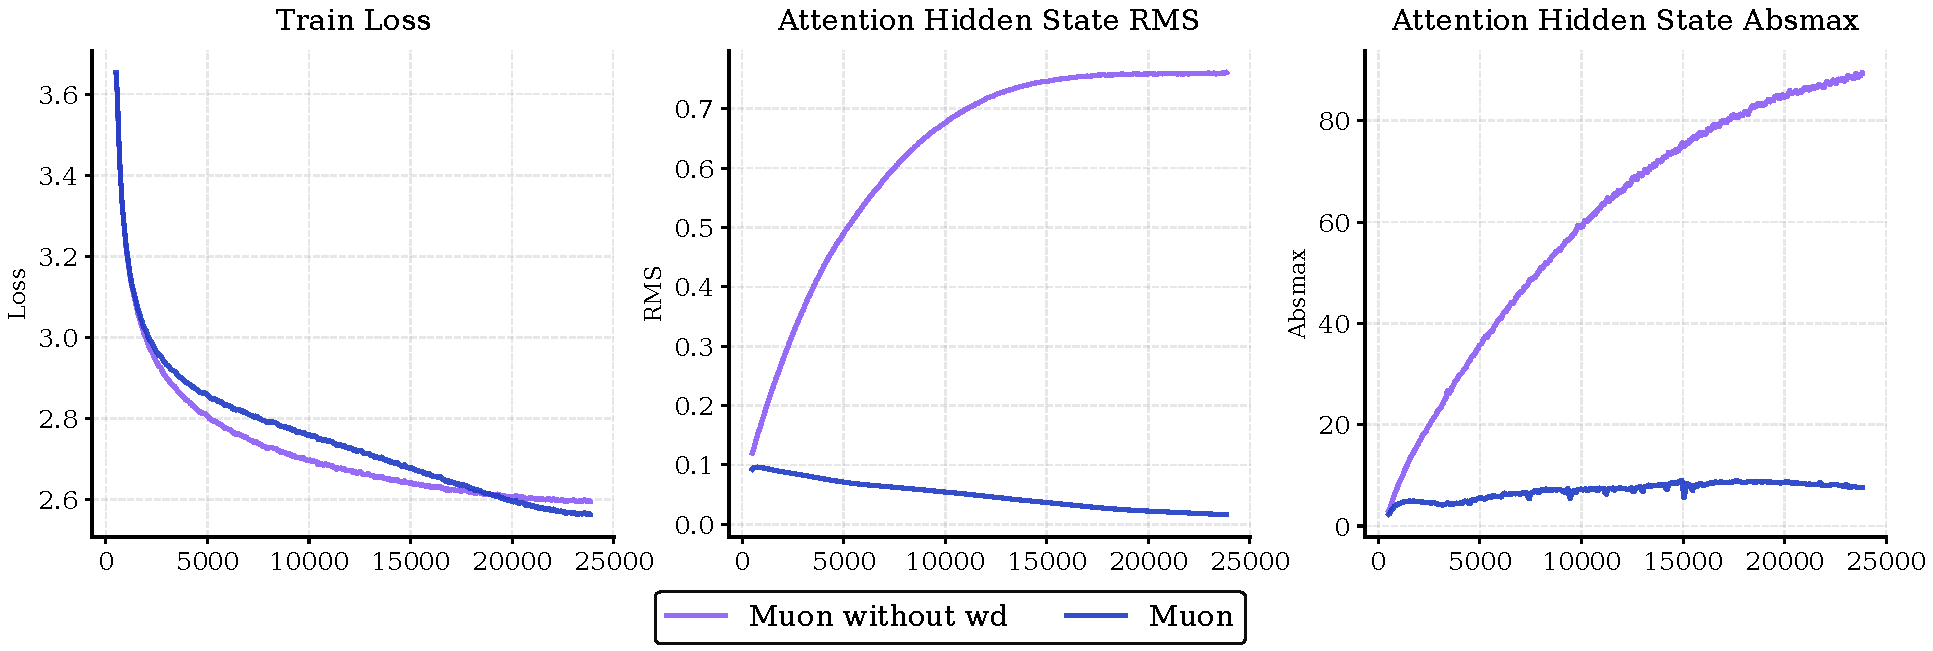
\includegraphics[width=\linewidth]{figures/details/weight_decay_triple_comparison.pdf}
    \caption{\textbf{Abaltion of weight decay in \textcolor{MuonColor}{Muon}.} In contrast with \textcolor{SpectralSphereColor}{Spectral Sphere} (\cref{fig:hidden_state_tracker}), without weight constraint, \textcolor{MuonColor}{Muon} training dynamics become instable, which in-turn would hurt performance.}
    \label{fig:muon_wd}
\end{figure}


In this section, we introduce spectral retraction mechanisms to counteract the accumulation of higher-order errors that may gradually drift the weights off the spectral sphere. As noted in~\cref{sec:retraction}, the remainder term $\mathcal{O}(\eta^2 R^2 \|\mPhi\|_2^2)$ in the Taylor expansion can accumulate over iterations. To enforce the exact constraint $\|\mW\|_2=R$ throughout training, we apply~\cref{eq:retraction_map} that projects the weights back onto the spectral manifold.

In practice, we consider two retraction variants that differ in how strictly the spectral constraint is enforced. The hard variant applies an explicit projection to maintain $\|\mW\|_2 = R$ at every step, while the dynamic variant replaces the exact projection with a soft, learning-rate-scaled radial correction that steers $\|\mW\|_2$ toward the target radius. These two variants correspond to enforcing the spectral constraint exactly or approximately, and lead to different interactions with conventional weight decay.

\paragraph{Hard retraction (exact projection).}
The hard variant applies the retraction map explicitly using an estimated top singular value $\sigma \approx \|\mW\|_2$ which is computed via Power Iteration.
\begin{equation}
\mW \gets \frac{R}{\sigma}\,\mW.
\end{equation}
This enforces the exact constraint $\|\mW\|_2 = R$ at every step, with deviations arising solely from the approximation error in $\sigma$.
Under this setting, Spectral Sphere is typically used together with standard decoupled weight decay as in AdamW: weight decay shrinks the full parameter vector, while the spectral retraction constrains the dominant singular value.

\paragraph{Dynamic retraction (soft spectral decay).}
The dynamic variant replaces the exact projection with a small, sign-controlled radial adjustment with hyperparameter $\lambda$.
\begin{equation}
\mW \gets \bigl(1 + \lambda\,\eta\sign(R-\sigma)\bigr)\mW.
\end{equation}
Instead of strictly enforcing the constraint $\|\mW\|_2 = R$, this update gently adjusts the spectral norm toward the target radius $R$ based on $\sigma$. Since the correction is proportional to $\eta$, the adjustment strength diminishes automatically as learning rate schedules. Under this formulation, dynamic retraction functions as a spectrally aligned, layer-wise analogue to decoupled weight decay. Consequently, we tie $\lambda$ to the AdamW weight decay coefficient and employ the dynamic variant as a drop-in replacement for conventional weight decay.

From a geometric perspective, the two variants above can both be viewed as approximate projections onto the spectral sphere. As discussed in~\cref{sec:retraction}, applying retraction at the beginning of iteration $t+1$ instead of after the update at iteration $t$ only introduces $\mathcal{O}(\eta^2)$ discrepancies. Consequently, the update remains first-order equivalent to steepest descent on the spectral manifold.

\subsection{MoE Routing Scaling Factor}
\label{app:moe_scaling}

Following~\citep{kexuefm-10945}, in our MoE architecture, the output $\vy$ is the sum of the shared experts and the routed experts. A critical issue arises from the magnitude mismatch between the two parts:
\begin{equation}
\vy = \underbrace{\sum_{i=1}^{N_{\text{shared}}} \ve_{\text{shared}, i}}_{\text{Weight } \approx 1} + \underbrace{\sum_{j \in \text{TopK}} g_j \ve_{\text{routed}, j}}_{\text{Weight } g_j \ll 1}
\end{equation}
The shared experts are directly added to the residual stream, effectively having a coefficient of 1. In contrast, the routed experts are multiplied by sigmoid probabilities $g_j$, which are typically small. Consequently, the variance (signal energy) of the routed experts is significantly lower than that of the shared experts, causing the optimizer to neglect the routed part.

To balance the contributions, we compute a scaling factor $M$ to the routed experts:
\begin{equation}
\vy = \sum_{i=1}^{N_{\text{shared}}} \ve_{\text{shared},i} + M \sum_{j\in\text{TopK}} g_j \ve_{\text{routed},j}
\end{equation}
We aim to choose $M$ such that the expected variance of the routed term matches that of the shared term, under assumption that experts have unit variance:
\begin{equation}
M \approx \sqrt{\frac{N_{\text{shared}}}{\mathbb{E}[\sum g_j^2]}}
\end{equation}
Using numerical simulation (\cref{lst:moe_scaling}) with $N_{\text{shared}}=1$ and Top-4 sigmoid routing, we find $M \approx 2.0$. We find this scaling factor is crucial for MoE training stability.

\begin{lstlisting}[
    style=Code,
    language=Python,
    caption={Python implementation for estimating the MoE scaling factor $M$.},
    label={lst:moe_scaling}
]
import numpy as np

def estimate_scaling_factor(n_total=64, k_routed=4, n_shared=1):
    factors = []
    for _ in range(10000):
        # 1. Simulate logits
        logits = np.random.randn(n_total - n_shared)

        # 2. Get Sigmoid Scores
        scores = 1 / (1 + np.exp(-logits))

        # 3. Select Top-K routed scores
        scores = np.sort(scores)[::-1][:k_routed]

        # 3. Normalize scores
        scores /= scores.sum()

        # 4. Calculate Magnitude
        magnitude = np.sum(scores**2)**0.5

        factors.append(n_shared**0.5 / magnitude)

    return np.mean(factors)
\end{lstlisting}

\subsection{\texorpdfstring{$\boldsymbol{\mu}$}{mu}P Width Scaling}
\label{app:mup_width}
In~\cref{fig:mup_width}, we conduct experiment to validate $\boldsymbol{\mu}$P width scaling across different model sizes from 70M to 1.8B. Additional AdamW results are included in~\cref{fig:triple_mup}.
We scale the hidden size, intermediate size, and number of attention heads (while fixing head dimensions). The models are trained on 30B tokens sampled from the Olmo2-mix-1124 dataset~\citep{olmo20252olmo2furious}. All optimizers use the Spectral $\boldsymbol{\mu}$P LR Scaler.

\begin{itemize}
    \item The LR is swept across \{1e-3, 3e-3, 5e-3, 7e-3, 9e-3, 1e-2, 1.5e-2, 2e-2, 3e-2\}.
    \item Hidden size is swept across \{256, 512, 1024, 2048\}.
\end{itemize}

\begin{figure}[ht]
    \centering
    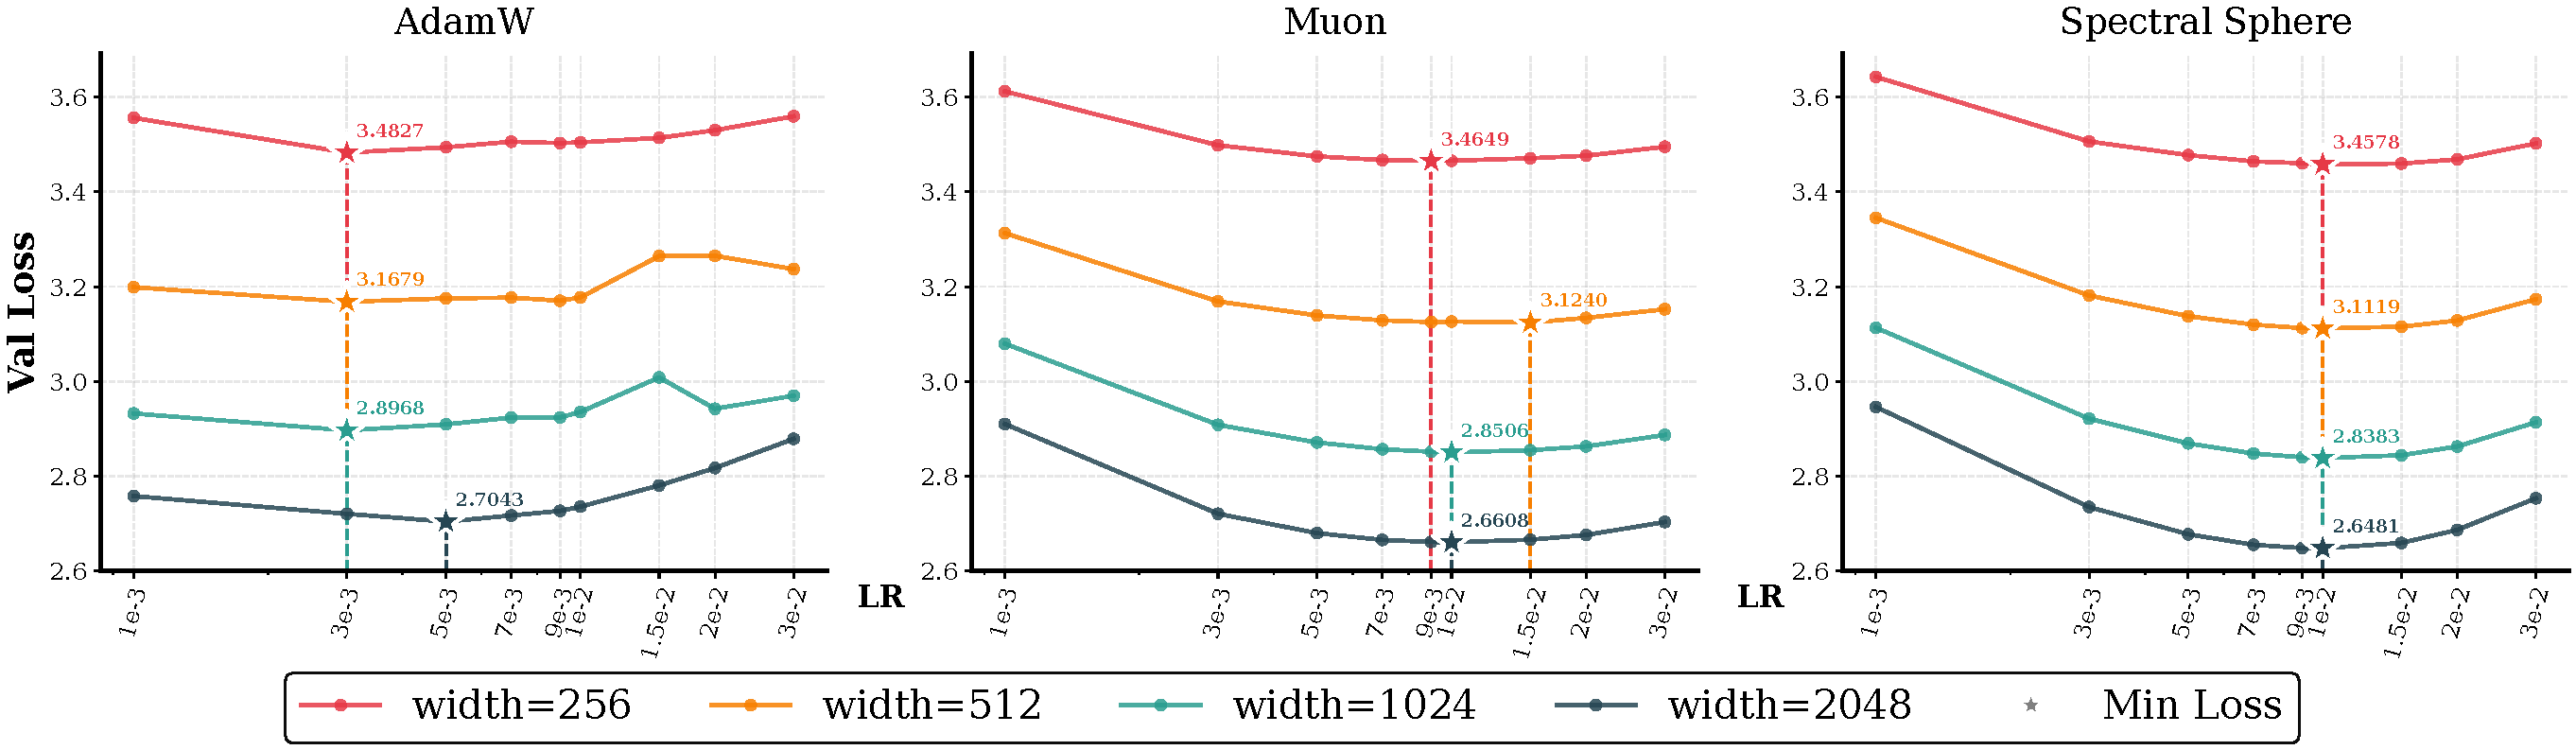
\includegraphics[width=1\linewidth]{figures/appendix/mup_triple_comparison.pdf}
    \caption{\textbf{$\boldsymbol{\mu}$P LR grid search with \textcolor{AdamWColor}{AdamW}, \textcolor{MuonColor}{Muon} and \textcolor{SpectralSphereColor}{Spectral Sphere}.} \textcolor{AdamWColor}{AdamW} shows even worse validation loss, with drifting optimal LR.}
    \label{fig:triple_mup}
\end{figure}
